% !TeX spellcheck = en_US
\documentclass[12pt]{article}


\usepackage[english]{babel}
\usepackage[utf8]{inputenc}
\usepackage{graphicx}
\usepackage{amsmath}
\usepackage{mathtools}
\usepackage{hyperref}
\usepackage{biblatex}
\usepackage{geometry}
\usepackage[hypcap]{caption}
\addbibresource{prediction.bib}

\hypersetup{
	colorlinks   = true,    % Colours links instead of ugly boxes
	urlcolor     = blue,    % Colour for external hyperlinks
	linkcolor    = blue,    % Colour of internal links
	citecolor    = red      % Colour of citations
}
\DeclarePairedDelimiter{\ceil}{\lceil}{\rceil}



%opening
\title{Predicting Traffic Patterns in\\ Software Defined Networks}

\author{
	Liva Giovanni - liva.giovanni@spes.uniud.it
	\and
	Hermann Hellwagner - hermann.hellwagner@itec.uni-klu.ac.at
	\and
	Marino Miculan - marino.miculan@uniud.it
}

\date{\today} 

\begin{document}
	
\maketitle

\begin{abstract}
	Just the prediction part
\end{abstract}

\newpage

\section{Introduction}
The predictability of network traffic is the main aim of the thesis. 
Usually, there are two different category of network prediction: short and long period predictions.
The short forecast is used to guess values in terms of seconds or minutes. 
Instead, the long one is adopted to estimate the future workload. 
Therefore, it favors the possibility to produce better planning and decision.
To be able to predict future load of a network, we have to create a model of its behaviors. 
On the changing of a model we have different characteristics such as the correctness of the prediction and its adaptability.


There are two type of models: \textbf{Supervised} and \textbf{Unsupervised}.
The \textit{Supervised} algorithms takes as a input a set of objects and the desired output. 
The set of objects it is called training data.
The learning algorithm analyzes the training data and produces an inferred function that its behavior is checked with the last input. 
The internal structure of the model is changed according to the error between the forecast and the desired result.
Instead, the \textit{Unsupervised} learning tries to find hidden structure in unlabeled data. 
The difference with the \textit{Supervised} learning algorithms is that there is no error or reward signal to evaluate a potential solution.


We focus over the long term prediction and only on supervised classifier.
The decision of which classifier chose has been taken conducting an experiment in a small simulated network. 
We simulate a normal scenario of daily network usage through a network of 4 nodes. 
We repeat the simulation thirty times collecting at each execution statistics of the links utilization in terms of network bandwidth and the load of the switches.
From this information, we have created different dataset changing the features used and the numbers of the last observations.
Then, we have tested the prediction precision and recall of different algorithm at the varying of the distinct datasets. 
\begin{figure}[h!]
	\centering
	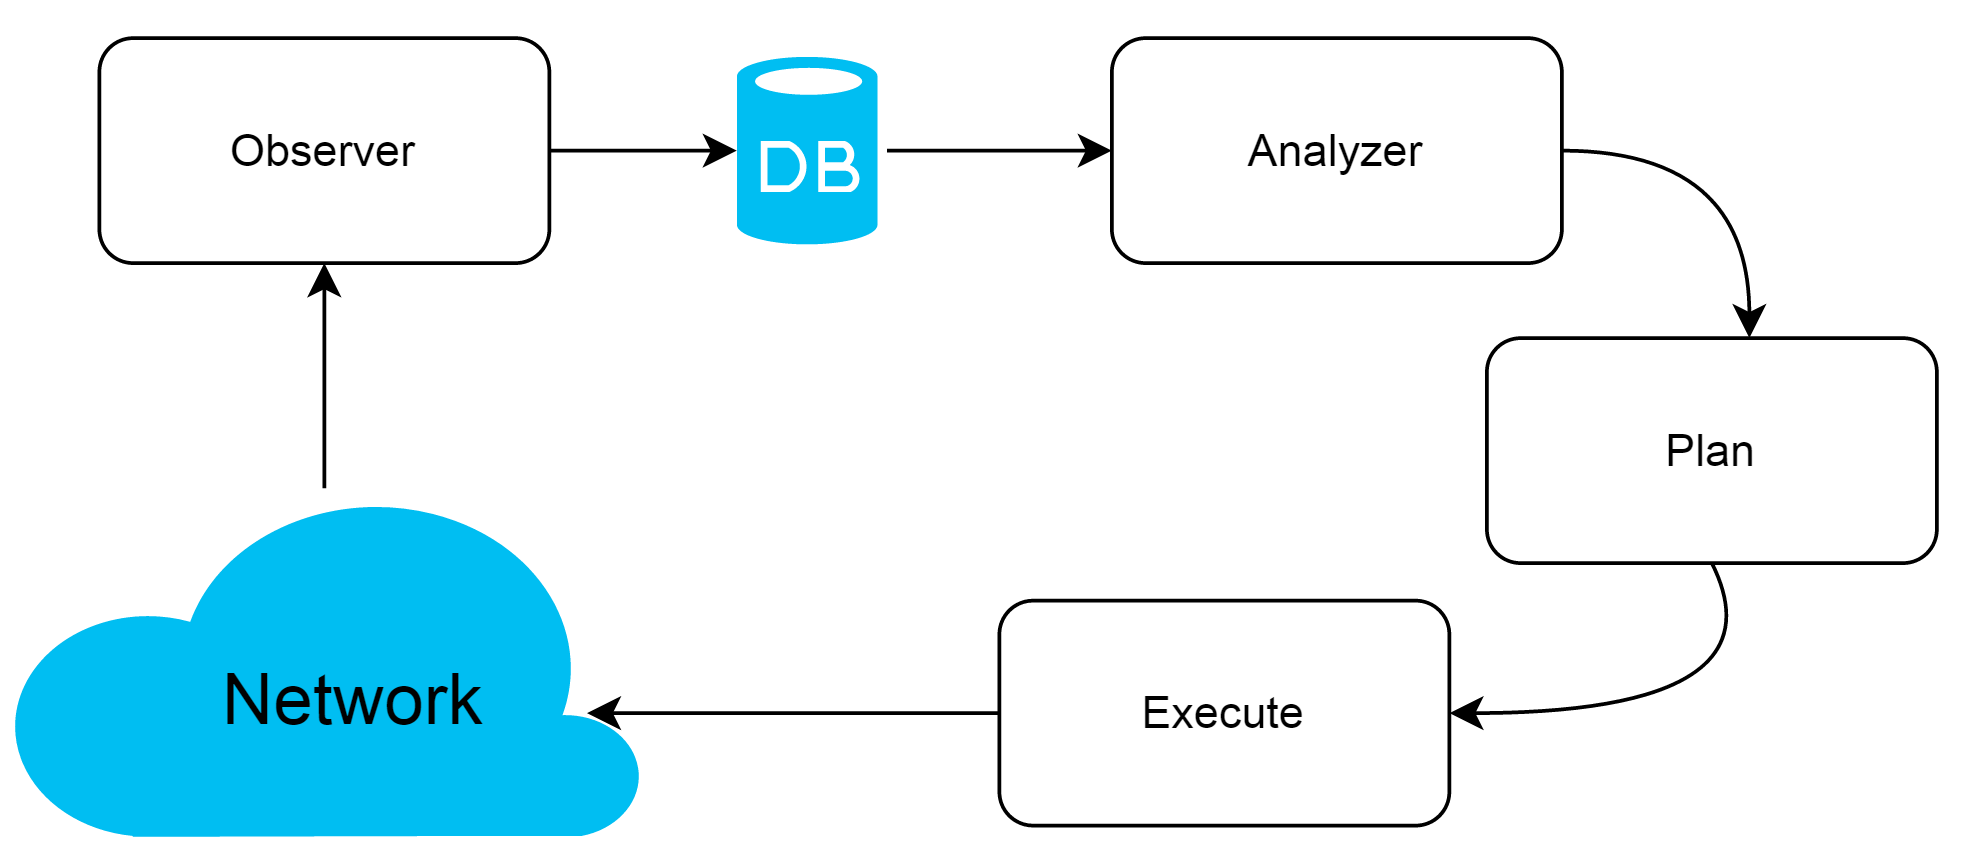
\includegraphics[width=1\textwidth]{img/predictionGraph.png}
	\caption[]
	{The different phases of the prediction}
	\label{fig:predictionConf}
\end{figure}


The implementation of the prediction is designed in four different phases
\begin{itemize}
	\item Observer
	\item Analyzing
	\item Plan
	\item Execute
\end{itemize}
A graphical representation of the interconnection between the four modules is given in Figure \ref{fig:predictionConf}.\\


\textbf{Observer}. It is implemented as a daemon in the cloud application. 
Every few minute it launches a python script which queries the network controller via 	\textit{REST API} and then stores the result inside a $nosql$ database.
The information saved regards the network load, switches and flows.



\textbf{Analyzing}. It is done looking through the information inside the database. 
A java application collects the data from the database and converts the knowledge in the Attribute-Relation File Format (ARFF). 
This format is an ASCII text file that describes a list of instances sharing a set of attributes.
The application depends on the $weka$ (Waikato Environment for Knowledge Analysis) package, a well known suite of learning machine algorithms developed by the University of Waikato.
The ARFF files are read by the weka package and used to produce the model that is adopted to make predictions.


\textbf{Plan}. It is demanded to the Administrator.
He or she can write rules to specify what to do when a particular event occurs.
In the cloud application the administrator has the possibility to create the rules that are stored inside the FloodLight controller.


\textbf{Execute}. It is implemented by the controller. 
It monitors the network and every few minutes it makes predictions using the previously generated model.
When it perceives from a forecast that some rules can be applied, it fires them.


Further, every module is uncoupled from the others. 
This design decision of modularity gives us the possibility to change or upgrade every module whenever there is the necessity.
This feature is crucial for the prediction phase.
We can test new classifiers or the addiction of new features in a separate and controlled network without affecting the production one. Moreover, we can hot swapping the model using the cloud interface.
We have designed the controller to work with a different model for each switch. 
This decision brings the possibility to predict when a particular node will be overloaded with more precision and recall.\\

 







\section{Prediction over the Network}
\subsection{Configuration}
We have set up a small simulation to decide which classifier algorithm works better for our purpose.
The candidates were the following:
\begin{itemize}
	\item $NaiveBayes$ \cite{naiveBayes}: is a classifier based on the Bayes theorem. It assumes independence between the features of the model. It is in the family of simple probabilistic classifiers.
	\item $SMO$ \cite{smo1,smo2,smo3}: It is an algorithm that employs the support vector machines. The classifier learns by solving an optimization problem.
	\item $BayesNet$ \cite{BayesNet}: It uses the K2 learning algorithm that is in the family of the Naive Bayes. It uses a hill climbing algorithm restricted by an order on the variables of the model.
	\item $MultilayerPerceptron$ \cite{MPL1,MPL2}: It is the most known application of the neural network that uses the back-propagation technique to adjust its internal structure.
	\item $J48$: It is a java implementation of the C4.5 \cite{j48} decision tree algorithm.
	\item $K^*$ ($KStar$) \cite{kstar}: It is an instance-based classifier. It classifies a new instance using the one that is more near to one it has learned in terms of entropy.
	\item $ZeroR$:  This is the dumbest classifier of the list. We have chosen to test it so we can measure other classifiers by how well they do compared to this minimal level of performance. Given a certain data set, ZeroR permits to find out what is the minimum performance we may expect.
\end{itemize}


\begin{figure}[h!]
	\centering
	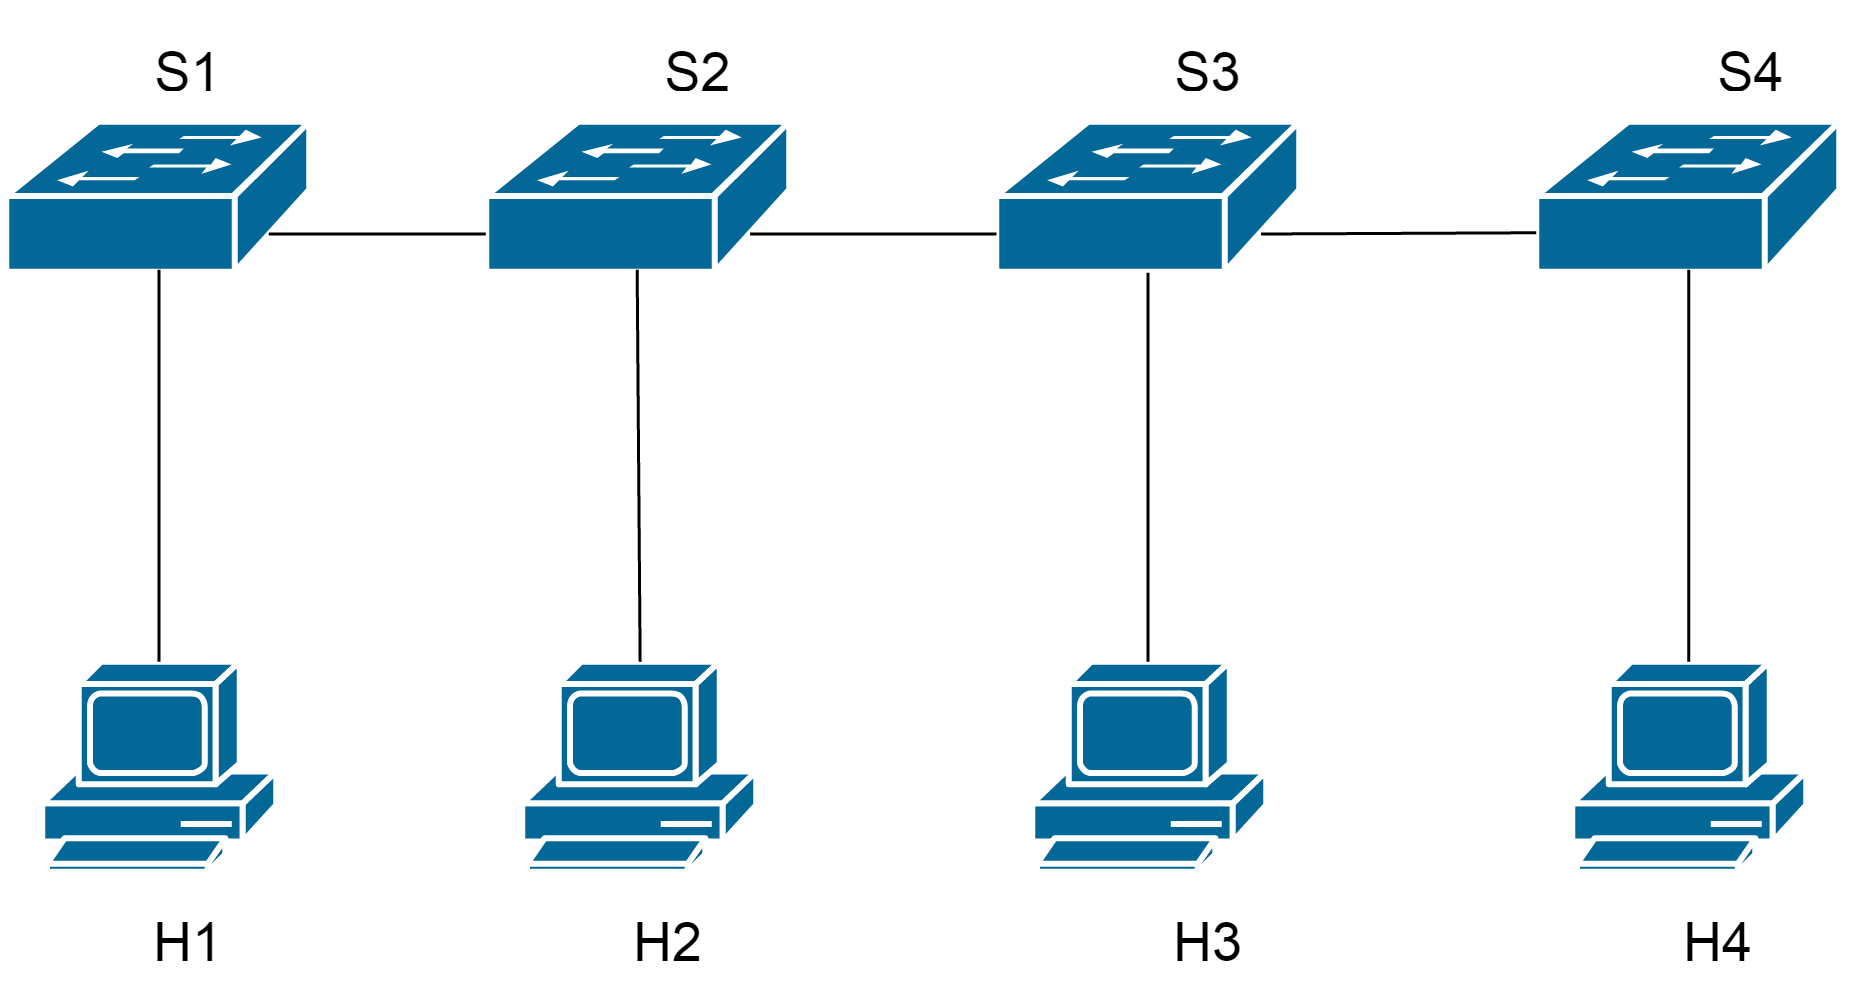
\includegraphics[width=.7\textwidth]{img/networkTopologyScenario.png}
	\caption[]
	{Topology of the network used to test the different classifiers}
	\label{fig:netScenatioTopo}
\end{figure}

\begin{figure}[h!]
	\centering
	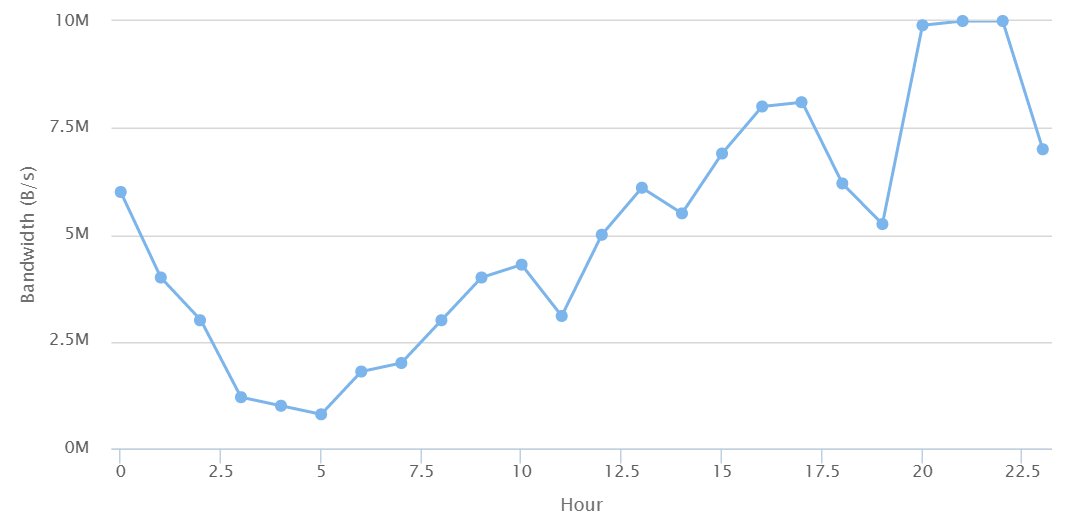
\includegraphics[width=0.9\textwidth]{img/networkScenario.png}
	\caption[]
	{Graph of the bandwidth simulation of a daily usage of the network}
	\label{fig:netScenarioConf}
\end{figure}


To found the most promising classifier, we have created a network of 4 nodes shows in Figure \ref{fig:netScenatioTopo}.
In this network we have generate traffic from the node $H1$ directed to $H4$ for a day respecting to the scenario predefined. The graph bandwidth generated is shown in Figure \ref{fig:netScenarioConf}.

The creation of the network relies on the virtualization of the hardware components.
Therefore, we have simulated it using Mininet \cite{mininet} with OpenFlow \cite{openflow} switches that have links of $10MB$ capacity.
The chosen controller is FloodLight \cite{floodlight}, an open source controller for Software Defined Network.


\subsection{DataSet}
In addiction to the decision of which classifier performs better, we have to find which information is most useful as a feature to the model to increase its prediction accuracy.
Our aim is to estimate the future load of the network in terms of bandwidth required. 
To be able to classify it correctly, we have stored the raw information taken from the controller inside intervals. 
Moreover, we have tested if the introduction of the derivative of the bandwidth helps or not the overall quality of the models.
The last variable investigated is the number of precedent measurements passed to the prediction module.
The results of our tests product five different datasets:
\begin{itemize}
	\item \textbf{200}: We use $200 KBytes$ as dimension of buckets and we use only the last 5 measurements of bandwidth.
	
	\item \textbf{500}: The size of the classes are of $500 KBytes$ and the remaining features are the same as before.
	
	\item \textbf{500\_D}: The intervals are $500 KBytes$ large, but now in addiction to the last 5 calculations we have the derivative between the consecutive values.

	\item \textbf{500\_D\_8}: The bucket are still of the same size but we increased the number of previous bandwidth to 8 values and we use the derivative.
	\item \textbf{500\_D\_10}: This configuration is the same as before, but the number of previous data is increased to 10.
\end{itemize}


\subsection{Evaluation}
The testing of the various datasets and classifiers is conducted using the classic ten fold cross validation.
Usually the classifiers are evaluated using the $RMSE = \sqrt{ \frac{ \sum_{t=1}^{n} (y(t) - \hat{y}(t))^2  }{n}  }$ where $y(t)$ is the real output and $\hat{y(t)}$ is the calculated one.
For our purpose, we have decided to take in account the maximal error in terms of distance between the class guessed and the real one.
This is possible because we can induce an order between classes since they correspond to a numerical range of Bytes. 
Moreover, we considered the average of this distance called $\sigma$.
We examined also the percentage score of the models to classify correctly the instances and the coverage.
The results of this evaluation are presented in the following tables.


\newpage 
\newgeometry{top=1.5cm,bottom=3cm}

\begin{table}[h!]
	\centering
	\resizebox{.8\textwidth}{!}{%
	\begin{tabular}{l|cccccccc}
	
& Max Error	&\% Correct	& $\sigma$	& RMSE		& Precision	& Recall	& Coverage (0.95) \\ \hline
NaiveBayes	& 23		& 34,33		& 3,31		& 0,1437	& 0,2756	& 0,2836	& 50,75  \\
SMO			& 27		& 33,59		& 3,52		& 0,1371	& 0,2207	& 0,3284	& 91,80  \\
ZeroR		& 45		& 10,45		& 23,52		& 0,1372	& 0,0109	& 0,1045	& 98,51  \\
BayesNet	& 19		& 37,31		& 3,30		& 0,1311	& 0,2738	& 0,3657	& 67,16  \\
MPL			& 43		& 35,82		& 3,90		& 0,1393	& 0,2626	& 0,2985	& 66,42  \\
J48			& 43		& 33,58		& 3,87		& 0,1399	& 0,3206	& 0,3582	& 45,52  \\
KStar		& 43		& 38,06		& 3,66		& 0,1579	& 0,2803	& 0,2985	& 40,30  \\
			
			
	\end{tabular}
	}
	\caption{Results for \textbf{200}}
	\label{tab:table_200}
\end{table}

\begin{table}[h!]
	\centering
	\resizebox{.8\textwidth}{!}{%
		\begin{tabular}{l|cccccccc}
			
& Max Error	&\% Correct	& $\sigma$	& RMSE		& Precision	& Recall	& Coverage (0.95) \\ \hline
NaiveBayes	& 9			& 50,75		& 1,27		& 0,1964	& 0,4763	& 0,4627	& 70,1493  \\
SMO			& 10		& 41,79		& 1,40		& 0,2064	& 0,3707	& 0,4478	& 97,7612  \\
ZeroR		& 18		& 10,45		& 9,10		& 0,2103	& 0,0215	& 0,1045	& 97,7612  \\
BayesNet	& 7			& 43,28		& 1,37		& 0,1881	& 0,4059	& 0,4776	& 82,0896  \\
MPL			& 17		& 48,51		& 1,31		& 0,2007	& 0,4359	& 0,4552	& 71,6418  \\
J48			& 17		& 49,25		& 1,35		& 0,2080	& 0,3914	& 0,4254	& 55,2239  \\
KStar		& 17		& 50,75		& 1,44		& 0,2204	& 0,4608	& 0,4403	& 53,7313  \\

			
		\end{tabular}
	}
	\caption{Results for \textbf{500}}
	\label{tab:table_500}
\end{table}

\begin{table}[h!]
	\centering
	\resizebox{.8\textwidth}{!}{%
		\begin{tabular}{l|cccccccc}
			
& Max Error	&\% Correct	& $\sigma$	& RMSE	& Precision	& Recall	& Coverage (0.95) \\ \hline

NaiveBayes	& 7		& 45,52		& 1,38		& 0,2105	& 0,4572	& 0,4478	& 56,7164 \\
SMO			& 10	& 41,79		& 1,40		& 0,2063	& 0,3813	& 0,4328	& 97,7612 \\
ZeroR		& 18	& 10,45		& 9,10		& 0,2103	& 0,0202	& 0,0896	& 97,7612 \\
BayesNet	& 7		& 43,28		& 1,37		& 0,1823	& 0,4809	& 0,5224	& 86,5672 \\
MPL			& 7		& 49,25		& 1,19		& 0,2035	& 0,4496	& 0,4478	& 67,9104 \\
J48			& 17	& 52,24		& 1,40		& 0,2026	& 0,4823	& 0,4701	& 64,9254 \\
KStar		& 9		& 41,04		& 1,54		& 0,2350	& 0,4428	& 0,4030	& 43,2836 \\
			
			
			
		\end{tabular}
	}
	\caption{Results for \textbf{500\_D}}
	\label{tab:table_500D}
\end{table}

\begin{table}[h!]
	\centering
	\resizebox{.8\textwidth}{!}{%
		\begin{tabular}{l|cccccccc}
			
& Max Error	&\% Correct	& $\sigma$	& RMSE	& Precision	& Recall	& Coverage (0.95) \\ \hline
			
		NaiveBayes	& 17	& 43,28		& 1,67		& 0,2216	& 0,4480	& 0,4328	& 52,2388 \\
		SMO			& 7		& 55,22		& 1,03		& 0,2056	& 0,6230	& 0,6493	& 99,2537 \\
		ZeroR		& 18	& 10,45		& 9,10		& 0,2103	& 0,0224	& 0,1119	& 97,7612 \\
		BayesNet	& 7		& 51,49		& 1,18		& 0,1794	& 0,4489	& 0,5299	& 76,8657 \\
		MPL			& 17	& 60,45		& 1,12		& 0,1746	& 0,6070	& 0,5821	& 75,3731 \\
		J48			& 17	& 58,96		& 1,25		& 0,1974	& 0,5071	& 0,5000	& 61,1940 \\
		KStar		& 17	& 40,30		& 1,95		& 0,2460	& 0,3735	& 0,3582	& 36,5672 \\
		
			
			
			
		\end{tabular}
	}
	\caption{Results for \textbf{500\_D\_8}}
	\label{tab:table_500D8}
\end{table}

\begin{table}[h!]
	\centering
	\resizebox{.8\textwidth}{!}{%
		\begin{tabular}{l|cccccccc}
			
& Max Error	&\% Correct	& $\sigma$	& RMSE	& Precision	& Recall	& Coverage (0.95) \\ \hline
			
NaiveBayes	& 8		& 38,81		& 1,67		& 0,2321	& 0,3503	& 0,3433	& 47,0149 \\
SMO			& 9		& 46,27		& 1,40		& 0,2064	& 0,3780	& 0,4328	& 98,5075 \\
ZeroR		& 18	& 10,45		& 9,10		& 0,2103	& 0,0190	& 0,0821	& 97,7612 \\
BayesNet	& 7		& 48,51		& 1,28		& 0,1932	& 0,4203	& 0,5000	& 72,3881 \\
MPL			& 17	& 47,01		& 1,49		& 0,2126	& 0,3819	& 0,3955	& 60,4478 \\
J48			& 8		& 43,28		& 1,37		& 0,2045	& 0,4201	& 0,4478	& 69,4030 \\
KStar		& 17	& 36,57		& 2,02		& 0,2601	& 0,3113	& 0,2836	& 28,3582 \\


			
		\end{tabular}
	}
	\caption{Results for \textbf{500\_D\_10}}
	\label{tab:table_500D10}
\end{table}

\restoregeometry


\subsection{Discussion}


\hspace{14pt} \textbf{Number of Classes}. 
The number of classes in the first dataset is $ \frac{10 \text{MB} } { 0.2 \text{MB}}  = 50$. 
In all the others the classes are $20$. 
A crucial design feature is to choose the right size of the intervals in which the classifier has to work with.
With wider range the model has less difficulties to correctly classify an instance and it makes better predictions. 
Nevertheless, this gives us less information because the forecasts are more general and tell us that the future traffic will fit in a bigger interval. With this knowledge we have less capacity of reaction. 
On the other hand, having smaller classes helps us to have more precise information in terms of future load, but these values are not trustworthy.
This behavior is confirmed comparing Table \ref{tab:table_200} with the others.

\textbf{Derivative}.

The introduction of the derivative as a feature passed to the model increase 

\textbf{Number of previous measurement}.

Avere 50\% di successo -> 10 volte meglio di sparare a caso $1/20 = 5\%$

\printbibliography 

	
\end{document}